En el oscilador del circuito de la figura \ref{3.0}, conocido como oscilador Colpitts, se desea calcular su frecuencia de oscilación $f_o$, el factor de calidad $Q_c$ y el valor de la corriente de polarización $I_{CQ}$ del transistor TBJ para que comiencen las oscilaciones.

\begin{figure}[H]
\centering
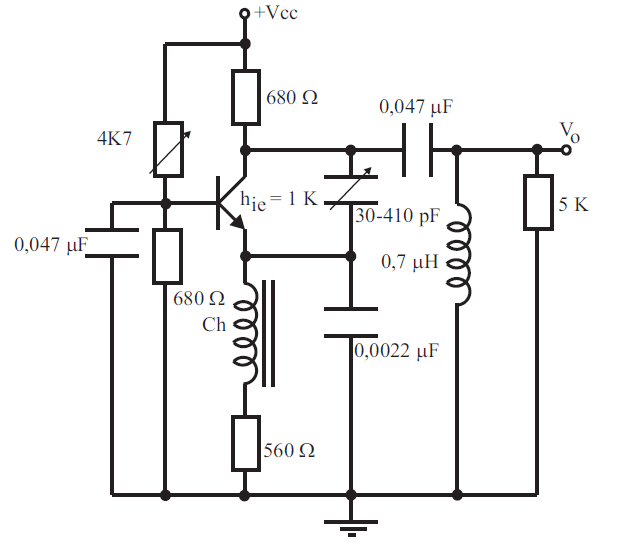
\includegraphics[width=0.5\linewidth]{images/circuito_2.png}
\caption{Oscilador tipo Colpitts.}
\label{3.0}
\end{figure}

Redibujando el circuito, para un análisis de alterna, donde los capacitores de desacople de $0.047 \mu f$ actúan como corto-circuitos, y la bobina de choque $Ch$ actúa como un circuito-abierto:

\begin{figure}[H]
  	\centering
		 \begin{circuitikz}[scale=1.5][american]
		 \draw
	     (0,0) 	node[npn,rotate=0](Q1){} node[]{}
	      ;
	      % Conectores
         \draw
	     (Q1.base) -- ++(-0.1,0) node[circ] node[above]{$V_t'$} -- ++(-1,0) -- ++(0,-1.5) -- ++(6,0) -- ++(0,2.77) -- (3,1.27){}
	     ;
	     \draw
	     (Q1.base) -- ++(-0.1,0) -- ++(0,-0.5) node[ground]
	     {};
	     
	     \draw 
	     (Q1.collector) -- (0,1.27) -- ++(1,0) node[circ] to [vC,l_=$C_1$]  ++(0,-2.05) node [circ] -- (0,-0.78) to (Q1.emitter){};
	     
	     \draw
	     (1,1.27) to [L,l_=$L$] (3,1.27) node[circ] to [C,l_=$C2$] (3,-0.78) -- (0,-0.78){} ;
	     
	     \draw 
	     (1,1.27) -- (1,2.2) to [R, l_=$R_L$] (3,2.2) -- (3,1.27) to ++(0.4,0)node[above]{$V_t$}{};
	    
		\end{circuitikz}
    \caption[Equivalente de alterna]{Equivalente de alterna.}
    \label{3.1}
\end{figure}

Donde $R_L=680 K\Omega \parallel 5 K \Omega$. En el circuito equivalente, es evidente que la red amplificadora $a(w)$ corresponde al transistor TBJ, quien desfasa $180\degree$ a la fase, por lo que la red selectiva de frecuencia ,$LC$, también debe desfasar la fase en $180\degree$. Se puede demostrar que para cumplir la condición de fase se tiene que cumplir la siguiente ecuación, que establece que la suma de las reactancias debe ser nula:

\begin{equation}
\label{eq:3.0}
X_L + X_{C_1} + X_{C_2} = 0
\end{equation}

Donde tal expresión se cumple para la siguiente frecuencia de oscilación:


\begin{equation}
\label{eq:3.1}
f_o = \frac{1}{2\pi} \cdot \sqrt{\frac{C_1 + C_2}{L\cdot C_1 \cdot C_2}}
\end{equation}

Pero dado que el capacitor $C_1$ varía entre $30 p F $ y   $410 p F $, la frecuencia $f_o$ varía entonces entre: 

\begin{equation}
 \label{eq:3.2}
   f_o= \left\{ \begin{array}{lcc}
             10.23 MHz &   si  & C_1 = 30 p F \\
             \\ 34.97 MHz &  si  & C_1 = 410 p F
             \end{array}
   \right. 
\end{equation}

Conociendo que la atenuación de la red $\beta(w)$ es $\frac{X_1}{X_2}=\frac{C_2}{C_1}$, la peor atenuación se da para el valor mínimo de $C_1$, es decir, el valor máximo de $f_o$, $34.97 MHz$. Se analiza entonces el circuito cortando el lazo entre los nodos $V_t$ y $V_t'$, como se observa en la figura \ref{3.2}.

\begin{figure}[H]
  	\centering
		 \begin{circuitikz}[scale=1.5][american]
		 \draw
	     (0,0) 	node[npn,rotate=0](Q1){} node[]{}
	      ;
	      % Conectores
         \draw
	     (Q1.base) -- ++(-0.1,0) node[ocirc] node[above]{$V_t'$} {} % -- ++(-1,0) -- ++(0,-1.5) -- ++(6,0) -- ++(0,2.77) -- (3,1.27){}
	     ;
	     %\draw
	     %(Q1.base) -- ++(-0.1,0) -- ++(0,-0.5) node[ground]
	     %{};
	     
	     \draw 
	     (Q1.collector) -- (0,1.27) -- ++(1,0) node[circ] to [vC,l_=$C_1$]  ++(0,-2.05) node [circ] -- (0,-0.78) to (Q1.emitter){};
	     
	     \draw
	     (1,1.27) to [L,l_=$L$] (3,1.27) node[circ] to [C,l_=$C2$] (3,-0.78) -- (0,-0.78){} ;
	     
	     \draw 
	     (1,1.27) -- (1,2.2) to [R, l_=$R_L$] (3,2.2) -- (3,1.27) to ++(0.4,0)node[above]{$V_t$} -- (4,1.27) to [R,l=$hie$] (4,-0.78) -- (3,-0.78) node[circ] {};
	    
		\end{circuitikz}
    \caption[Equivalente de alterna]{Equivalente de alterna a lazo abierto.}
    \label{3.2}
\end{figure}

Se debe probar la condición de amplitud: $\frac{V_t}{V_t'} = 1$. Se calcula la impedancia que ve el capacitor $C_1$ a la frecuencia $w_o=2\pi\cdot f_o(max)$:

\begin{equation}
\label{eq:3.3}
Z_{eq} = R_L\parallel X_L + hie\parallel X_{C_2} \approxeq 37 \Omega+ j\cdot142.3 \Omega
\end{equation}

Trabajando en términos de admitancia:

\begin{equation}
\label{eq:3.4}
Y_{eq} = \frac{1}{Z_{eq}} \approxeq 1.7 m \mho -j\cdot 6.6 m \mho \equiv \frac{1}{R_{eq}} -j\cdot \frac{1}{w_o\cdot L_{eq}} 
\end{equation}

De esta forma se obtienen, en paralelo a $C_1$, una resistencia equivalente $R_{eq}\approxeq 582 \Omega$ y un inductor equivalente $L{eq} \approxeq 691 n Hy$. En el circuito de la figura \ref{3.3} se observa esta equivalencia: 

\begin{figure}[H]
  	\centering
		 \begin{circuitikz}[scale=1.5][american]
		 \draw
	     (0,0) 	node[npn,rotate=0](Q1){} node[]{}
	      ;
	      % Conectores
         \draw
	     (Q1.base) -- ++(-0.1,0) node[ocirc] node[above]{$V_t'$} {} % -- ++(-1,0) -- ++(0,-1.5) -- ++(6,0) -- ++(0,2.77) -- (3,1.27){}
	     ;
	     %\draw
	     %(Q1.base) -- ++(-0.1,0) -- ++(0,-0.5) node[ground]
	     %{};
	     
	     \draw 
	     (Q1.collector) -- (0,1.27) -- ++(1,0) node[circ] to [vC,l_=$C_1$]  ++(0,-2.05) node [circ] -- (0,-0.78) to (Q1.emitter){};
	     
	     \draw
	     (1,1.27) -- (2,1.27) node[circ] to [L,l_=$L_{eq}$] (2,-0.78) -- (0,-0.78){} ;
	     
	     \draw 
	    (2,1.27) -- (3,1.27)  to [R,l=$R_{eq}$] (3,-0.78) -- (2,-0.78) node[circ] {};
	    
		\end{circuitikz}
    \caption[Equivalente de alterna]{Equivalente de thevenin.}
    \label{3.3}
\end{figure}

Por lo que la frecuencia de oscilación es:

\begin{equation}
\label{eq:3.5}
f_o' = \frac{1}{2\pi} \cdot \frac{1}{\sqrt{L{eq} \cdot C_1(min)}} \approxeq 34.95 MHz
\end{equation}

Se demuestra entonces que la frecuencia no se ve afectada al tener en cuenta los efectos de carga. Como un cálculo adicional se obtiene el factor de calidad de dicha red:

\begin{equation}
\label{eq:3.6}
Q_c = \frac{R_{eq}}{X_L} = \frac{R_{eq}}{2\pi \cdot f_o' \cdot L_{eq}} \approxeq 3.83
\end{equation}

Ahora bien, se sabe que la ganancia del transistor TBJ es:

\begin{equation}
\label{eq:3.7}
g_m \cdot R_{eq} = \frac{I_C}{V_T (2.6 mV)} \dot R_{eq}
\end{equation}

Sabiendo que la condición de arranque es que la ganancia del amplificador sea mayor a la atenuación de la red selectiva, se despeja el valor de la corriente del colector $I_C$ (polarización):

\begin{equation}
\label{eq:3.8}
 \frac{I_C}{V_T (2.6 mV)} \dot R_{eq} > \frac{C_2}{C_1 (min)}
\end{equation}

De esta forma se obtiene: $I_C > 3.3 mA$. Es decir, se debe de polarizar al transistor TBJ de forma tal de tener una corriente de colector que satisfaga la condición impuesta para que el circuito efectivamente funcione como un oscilador.